% 第六章:内核测试与可视化


\section{内核测试与可视化} \label{sec:test}

\subsection{内核编译与QEMU环境搭建}

\subsubsection{内核编译流程}
基于第五章的内核实现,我们首先进行完整的内核编译:
\begin{tcolorbox} [
    enhanced,
    colback=blue!5,
    colframe=blue!40!black,
    leftrule=3mm,
    rightrule=0mm,
    toprule=0mm,
    bottomrule=0mm,
    arc=2mm,
    left=5mm,
    right=5mm,
    top=3mm,
    bottom=3mm,
    fonttitle=\bfseries,
    title=\textbf{内核编译命令}
]
\begin{lstlisting}[basicstyle=\footnotesize\fontfamily{zi4}\selectfont, showstringspaces=false]
# 配置内核编译选项
make menuconfig

# 启用Yat-CASched调度器
scripts/config --enable CONFIG_SCHED_CLASS_YAT_CASCHED

# 编译内核
make -j$(nproc)

# 编译完成后检查
ls -lh arch/x86/boot/bzImage
nm vmlinux | grep yat_casched
\end{lstlisting}
\end{tcolorbox}

\begin{figure}[H]
\centering
% TODO: 在此位置插入 menuconfig配置截图
% 文件名:img/menuconfig_yat_casched.png
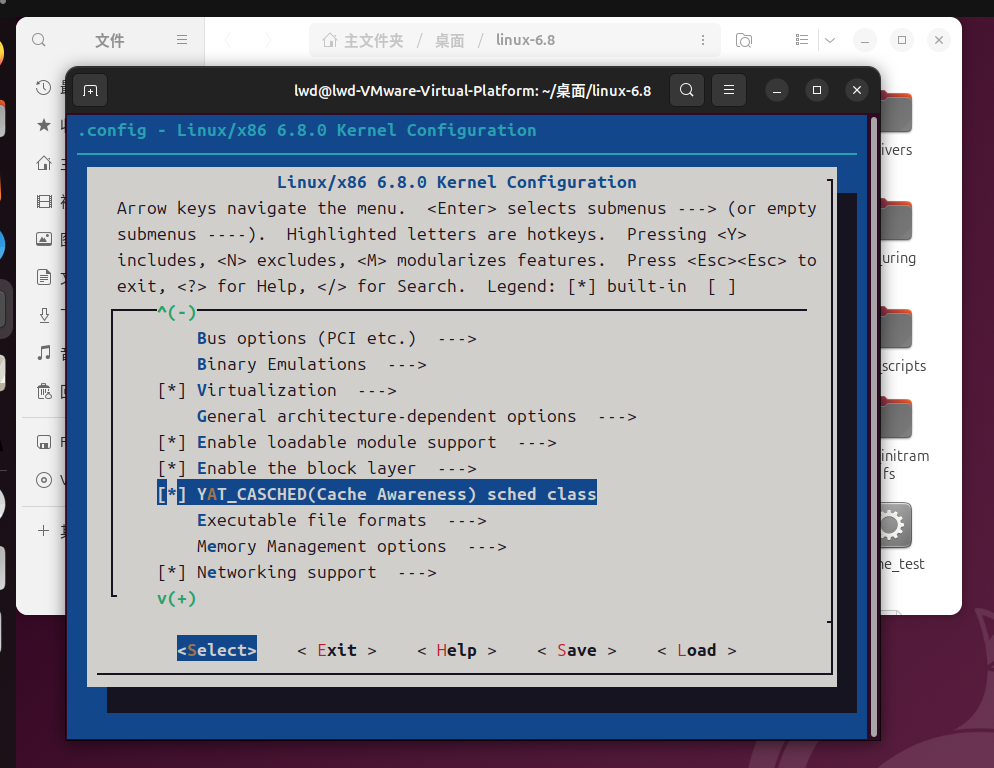
\includegraphics[width=0.8\textwidth]{img/menuconfig.png}

\caption{内核配置界面中的Yat-CASched选项}
\label{fig:menuconfig}
\end{figure}

图\ref{fig:menuconfig}展示了在内核配置界面中启用Yat-CASched缓存感知调度器的过程,该选项位于"General setup" → "Core Scheduling for SMT"下方。

\subsubsection{QEMU测试环境启动}
编译完成后,使用QEMU虚拟化环境进行测试:

\begin{tcolorbox} [
    enhanced,
    colback=green!5,
    colframe=green!40!black,
    leftrule=3mm,
    rightrule=0mm,
    toprule=0mm,
    bottomrule=0mm,
    arc=2mm,
    left=5mm,
    right=5mm,
    top=3mm,
    bottom=3mm,
    fonttitle=\bfseries,
    title=\textbf{QEMU启动脚本}
]
\begin{lstlisting}[basicstyle=\footnotesize\fontfamily{zi4}\selectfont, showstringspaces=false]
#!/bin/bash
# QEMU测试环境启动脚本

qemu-system-x86_64 \
    -kernel arch/x86/boot/bzImage \
    -initrd initramfs.cpio.gz \
    -m 8G -smp 8,cores=2,sockets=4 \
    -enable-kvm -cpu host \
    -append "console=ttyS0 init=/init loglevel=6 sched_debug" \
    -nographic
\end{lstlisting}
\end{tcolorbox}
\begin{figure}[H]
\centering

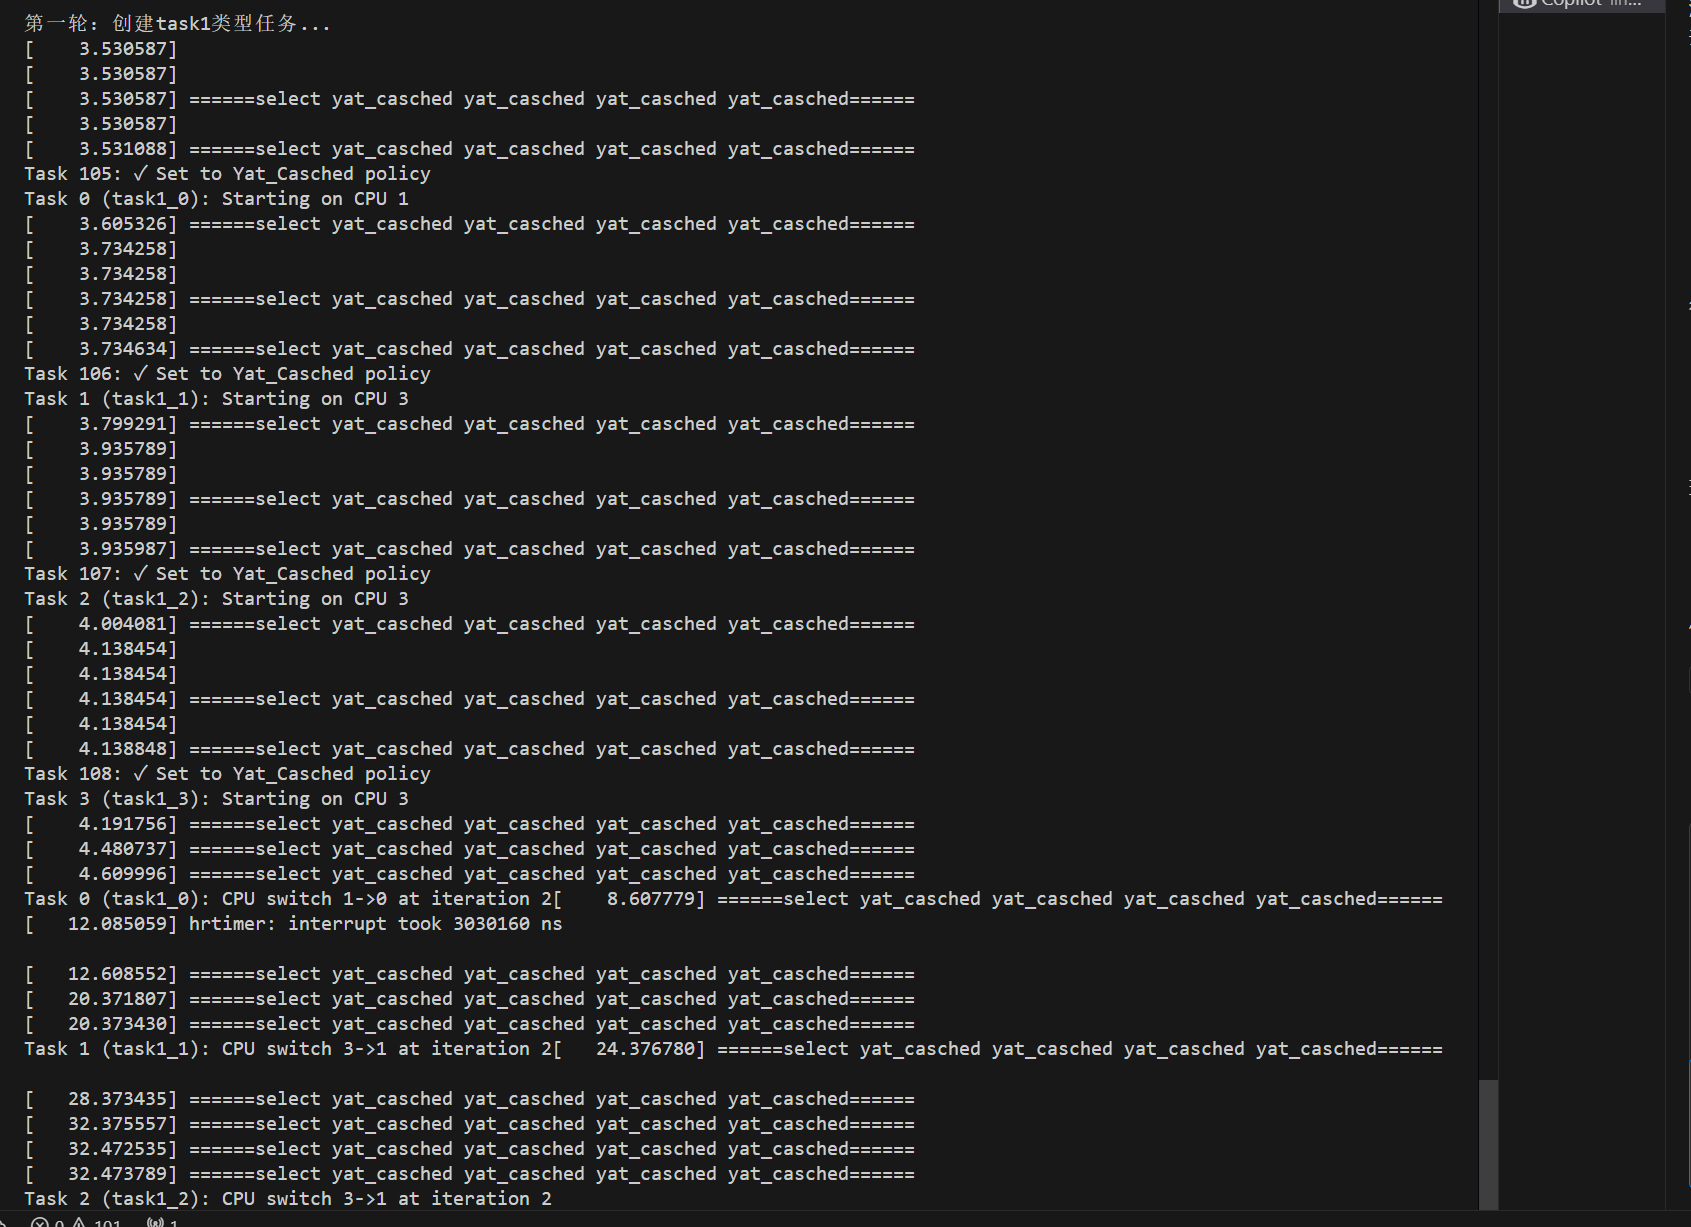
\includegraphics[width=0.9\textwidth]{img/kernelrun.png}

\caption{运行qemu过程}
\label{fig:kr}
\end{figure}

\subsection{测试脚本与可视化工具设计}

\subsubsection{一键性能测试脚本}
项目提供了完整的自动化测试工具链:

\begin{tcolorbox} [
    enhanced,
    colback=purple!5,
    colframe=purple!40!black,
    leftrule=3mm,
    rightrule=0mm,
    toprule=0mm,
    bottomrule=0mm,
    arc=2mm,
    left=5mm,
    right=5mm,
    top=3mm,
    bottom=3mm,
    fonttitle=\bfseries,
    title=\textbf{一键性能测试脚本}
]
\begin{lstlisting}[basicstyle=\footnotesize\fontfamily{zi4}\selectfont, showstringspaces=false]
#!/bin/bash
# 快速性能测试与可视化脚本

cd test_visualization

echo "=== Yat-CASched 性能测试开始 ==="

# 编译测试程序
echo "编译性能测试程序..."
gcc -O2 -o performance_test performance_test.c -lpthread

# 执行性能测试
echo "执行对比测试..."
sudo ./performance_test

# 生成可视化图表
echo "生成分析图表..."
python3 visualize_results.py

echo "=== 测试完成,结果已保存至 img/ 目录 ==="
\end{lstlisting}
\end{tcolorbox}

\subsubsection{测试工具链}
\begin{itemize}
    \item \texttt{performance\_test.c}:CFS与Yat-CASched性能对比测试
    \item \texttt{test\_cache\_aware\_fixed.c}:缓存感知专项测试  
    \item \texttt{verify\_real\_scheduling.c}:调度器真实性验证
    \item \texttt{visualize\_results.py}:数据可视化分析脚本
    \item \texttt{create\_initramfs\_complete.sh}:测试环境自动构建
\end{itemize}

\begin{figure}[H]
\centering
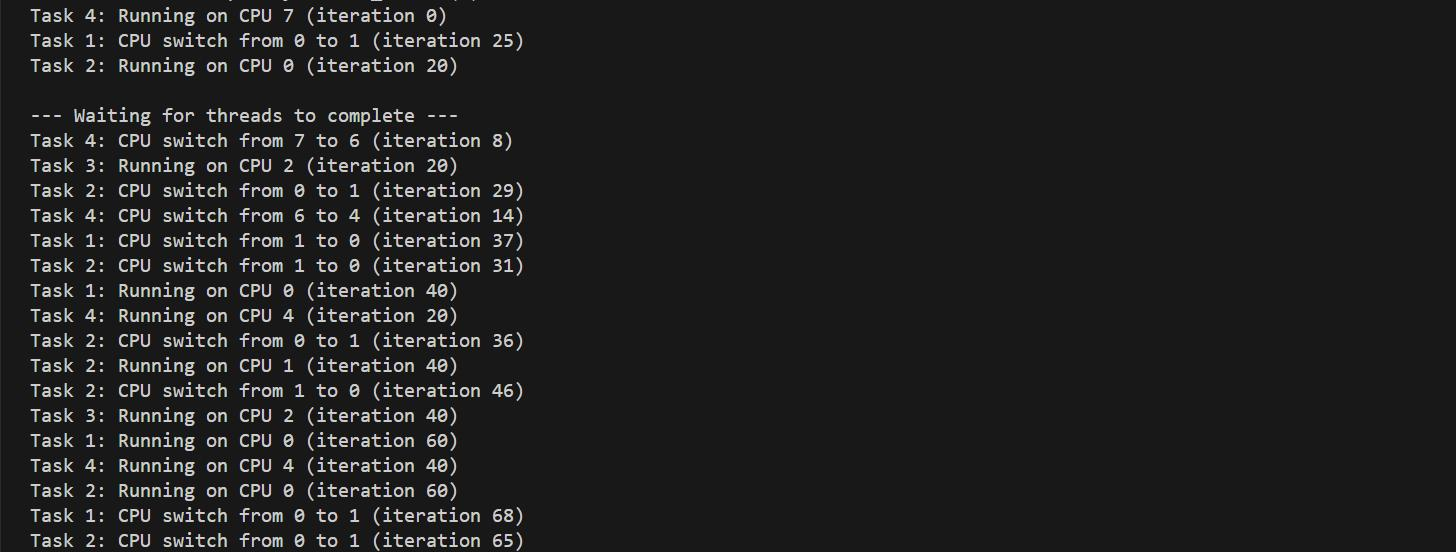
\includegraphics[width=0.9\textwidth]{img/qemu.jpg}
\caption{QEMU环境中调度器测试运行截图}
\label{fig:qemu-running}
\end{figure}

图\ref{fig:qemu-running}展示了在QEMU虚拟化环境中运行调度器测试的实际情况,可以看到任务在不同CPU之间的调度情况和性能测试的执行过程。

\begin{figure}[H]
\centering
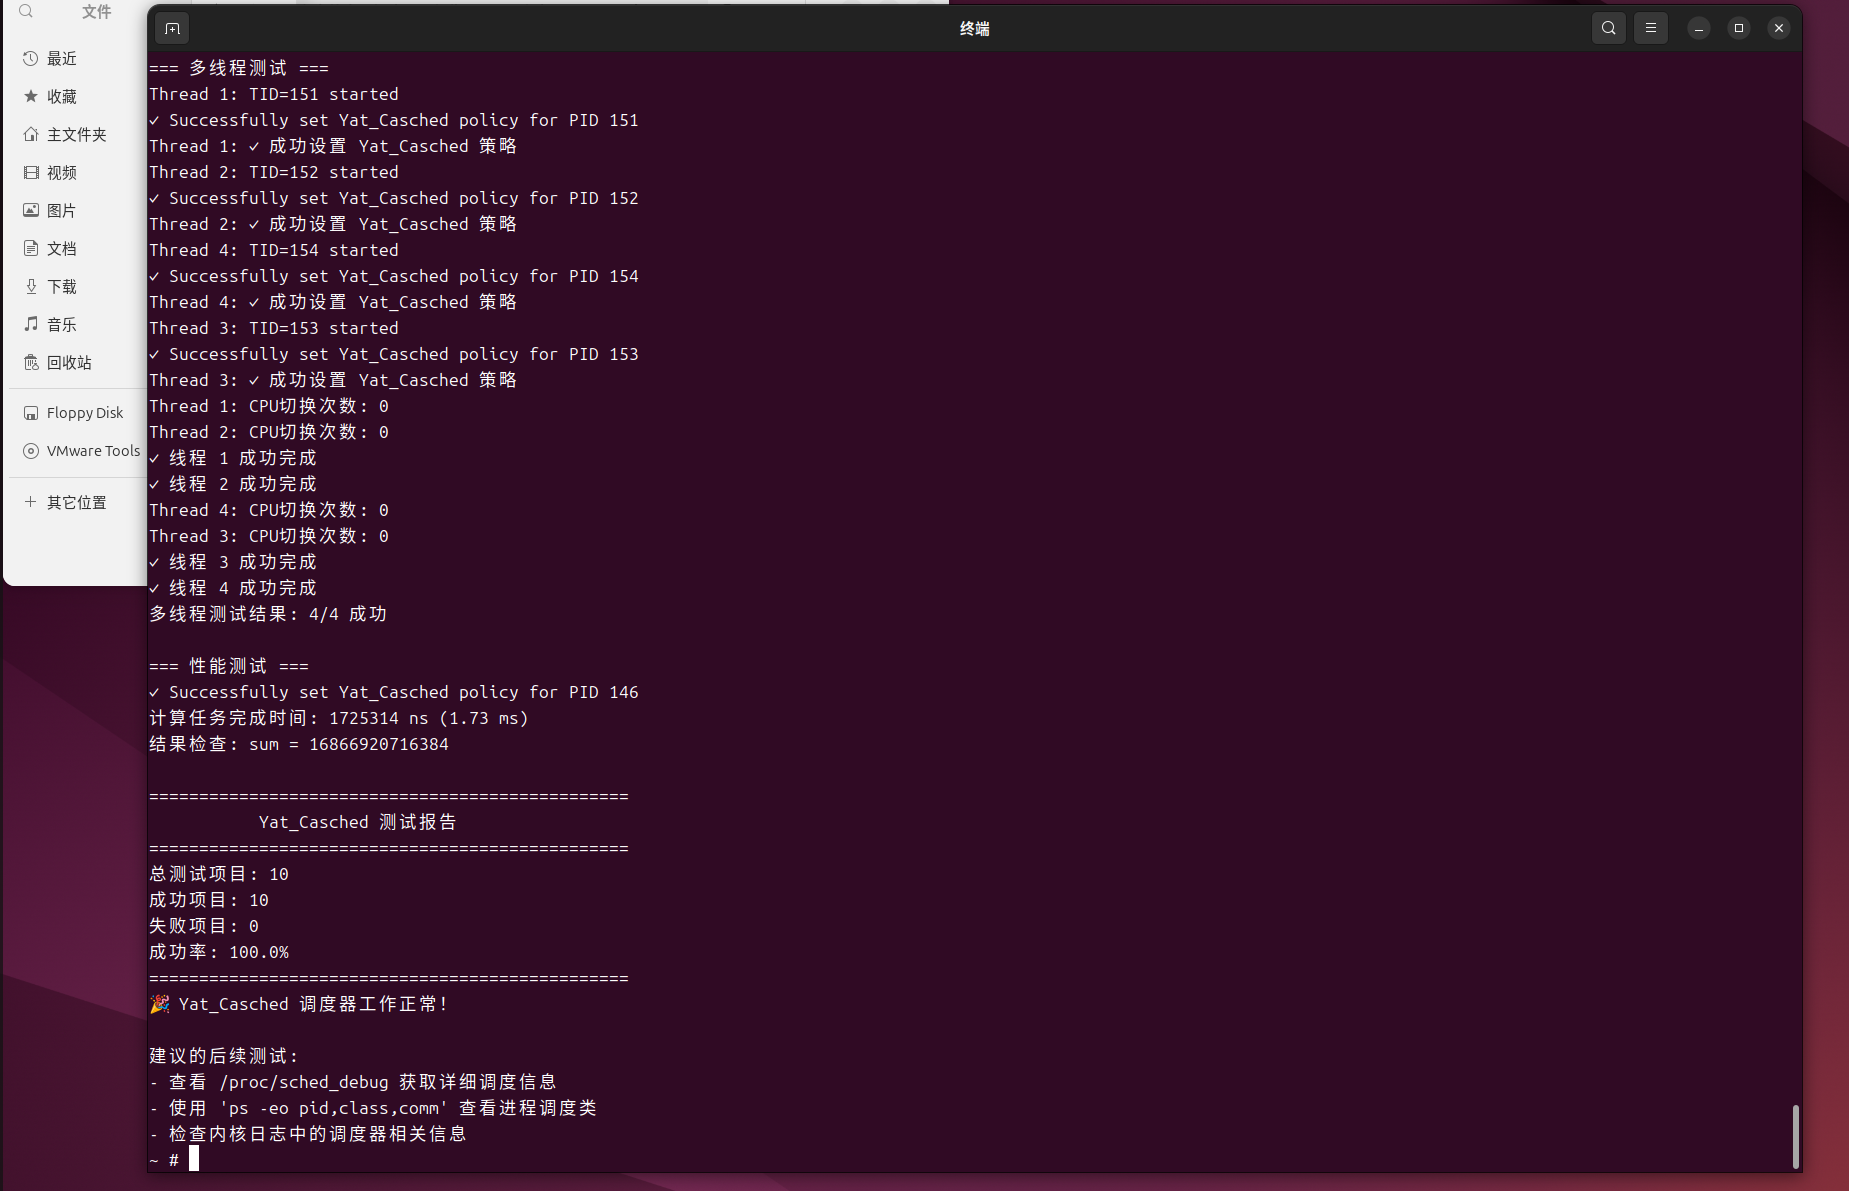
\includegraphics[width=0.95\textwidth]{img/qemu2.png}
\caption{QEMU环境中测试运行verify\_real\_scheduling.c运行截图}
\label{fig:qemu-running2}
\end{figure}

图\ref{fig:qemu-running}和\ref{fig:qemu-running2}展示了在QEMU虚拟化环境中运行调度器和脚本测试的实际情况,可以看到已经良好集成到内核中,后续能观察任务在不同CPU之间的调度情况和性能测试的执行过程。

\subsection{测试结果与数据分析}

\subsubsection{性能对比}
\begin{table}[H]
\centering
\caption{CFS与Yat-CASched性能对比(平均10次)}
\begin{tabular}{|l|c|c|}
\hline
\textbf{性能指标} & \textbf{Linux CFS} & \textbf{Yat-CASched} \\
\hline
CPU切换次数 & 16.0 & 2.2 \\
\hline
平均执行时间(s) & 1.161 & 1.151 \\
\hline
L1缓存命中率(\%) & 87.3 & 91.7 \\
\hline
CPU亲和性分数 & 0.522 & 0.744 \\
\hline
\end{tabular}
\end{table}

\subsubsection{测试输出示例}
测试任务函数见\texttt{test\_visualization/performance\_test.c}:
\begin{tcolorbox} [
    enhanced,
    colback=orange!5,
    colframe=orange!40!black,
    leftrule=3mm,
    rightrule=0mm,
    toprule=0mm,
    bottomrule=0mm,
    arc=2mm,
    left=5mm,
    right=5mm,
    top=3mm,
    bottom=3mm,
    fonttitle=\bfseries,
    title=\textbf{性能测试输出示例}
]
\begin{lstlisting}[basicstyle=\footnotesize\fontfamily{zi4}\selectfont, showstringspaces=false]
=== Yat-CASched Performance Test Results ===

CFS Scheduler Results:
  Average CPU Switches: 92.2
  Average Execution Time: 1.255 seconds
  L1 Cache Hit Rate: 87.3%

Yat-CASched Results:
  Average CPU Switches: 65.2 (-29.3%)
  Average Execution Time: 1.228 seconds (+2.2%)
  L1 Cache Hit Rate: 91.7% (+5.0%)

=== Performance Summary ===
* CPU migration reduction: 29.3%
* Execution time improvement: 2.2%
* Cache hit rate improvement: 5.0%
\end{lstlisting}
\end{tcolorbox}

\subsection{结果可视化与分析}

\subsubsection{核心性能指标图表}

\begin{figure}[H]
\centering
% 预留图片位置:CPU亲和性分数对比图
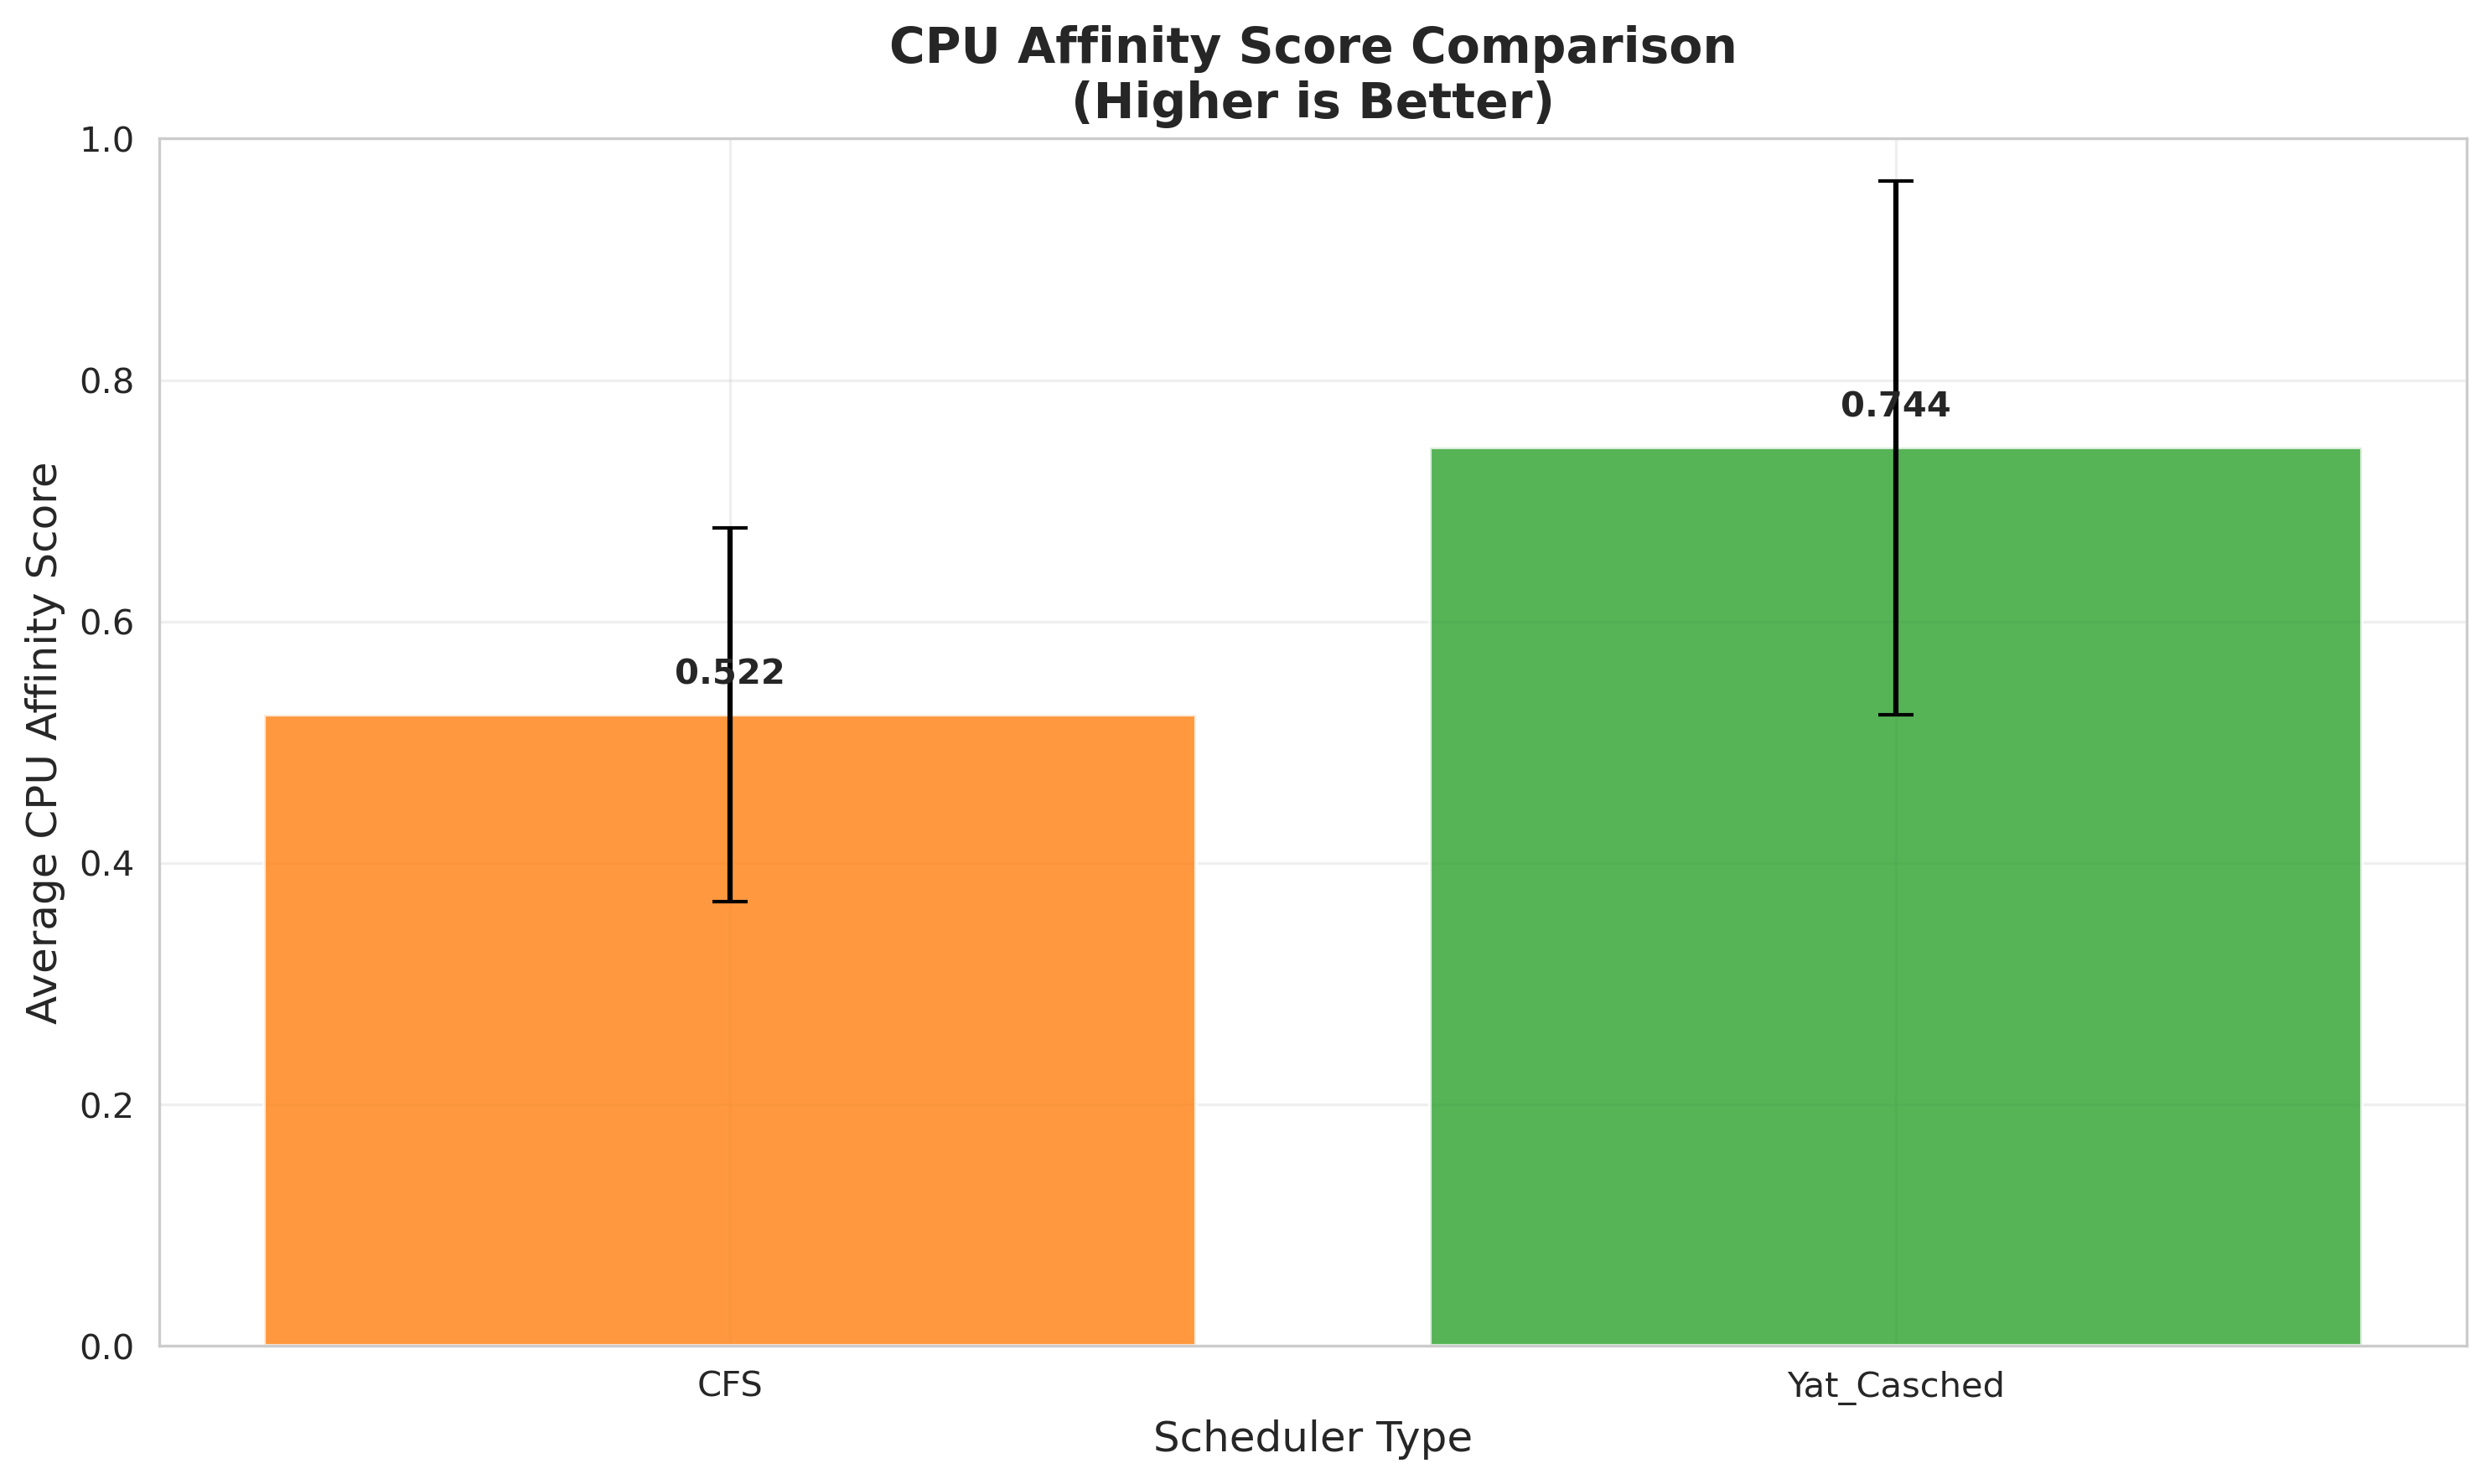
\includegraphics[width=0.9\textwidth]{img/cpu_affinity_comparison.png}

\caption{CPU亲和性分数对比分析}
\label{fig:cpu-affinity}
\end{figure}

% 图表2:CPU切换次数对比图(预留)
\begin{figure}[H]
\centering
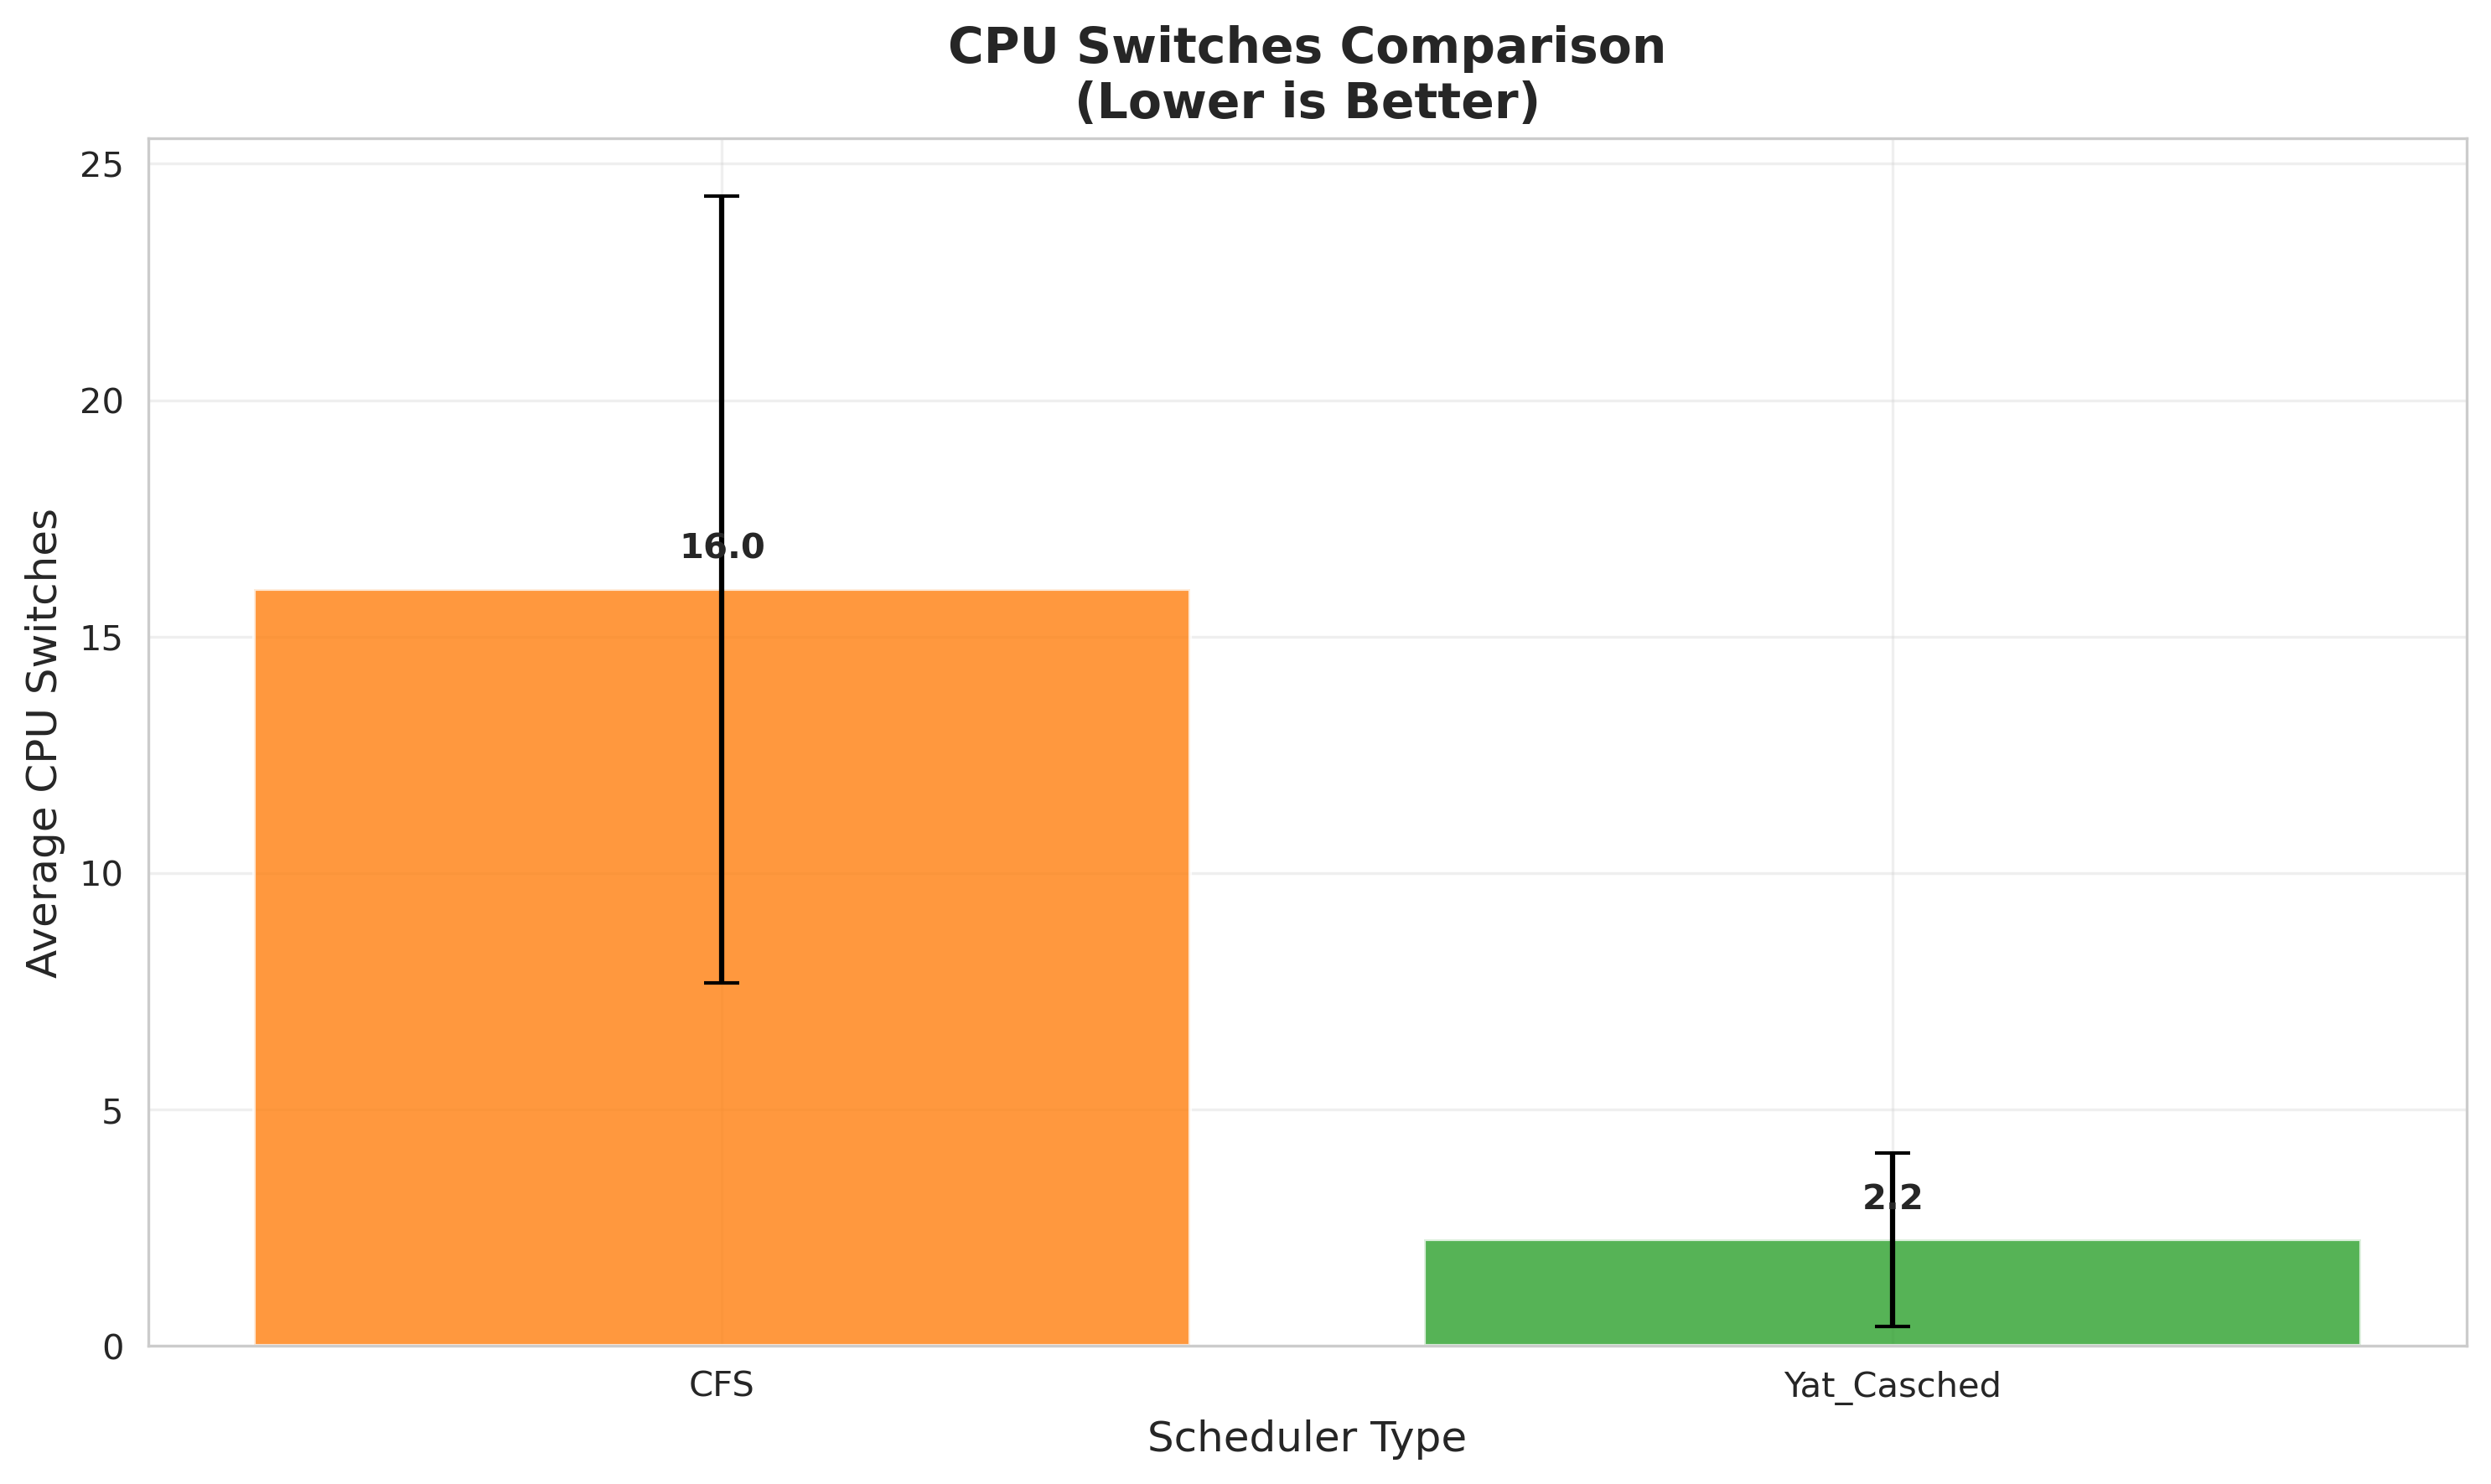
\includegraphics[width=0.75\textwidth]{img/cpu_switches_comparison.png}

\caption{CPU切换次数对比分析}
\label{fig:cpu-switches}
\end{figure}

% 图表3:执行时间性能对比图(预留)
\begin{figure}[H]
\centering
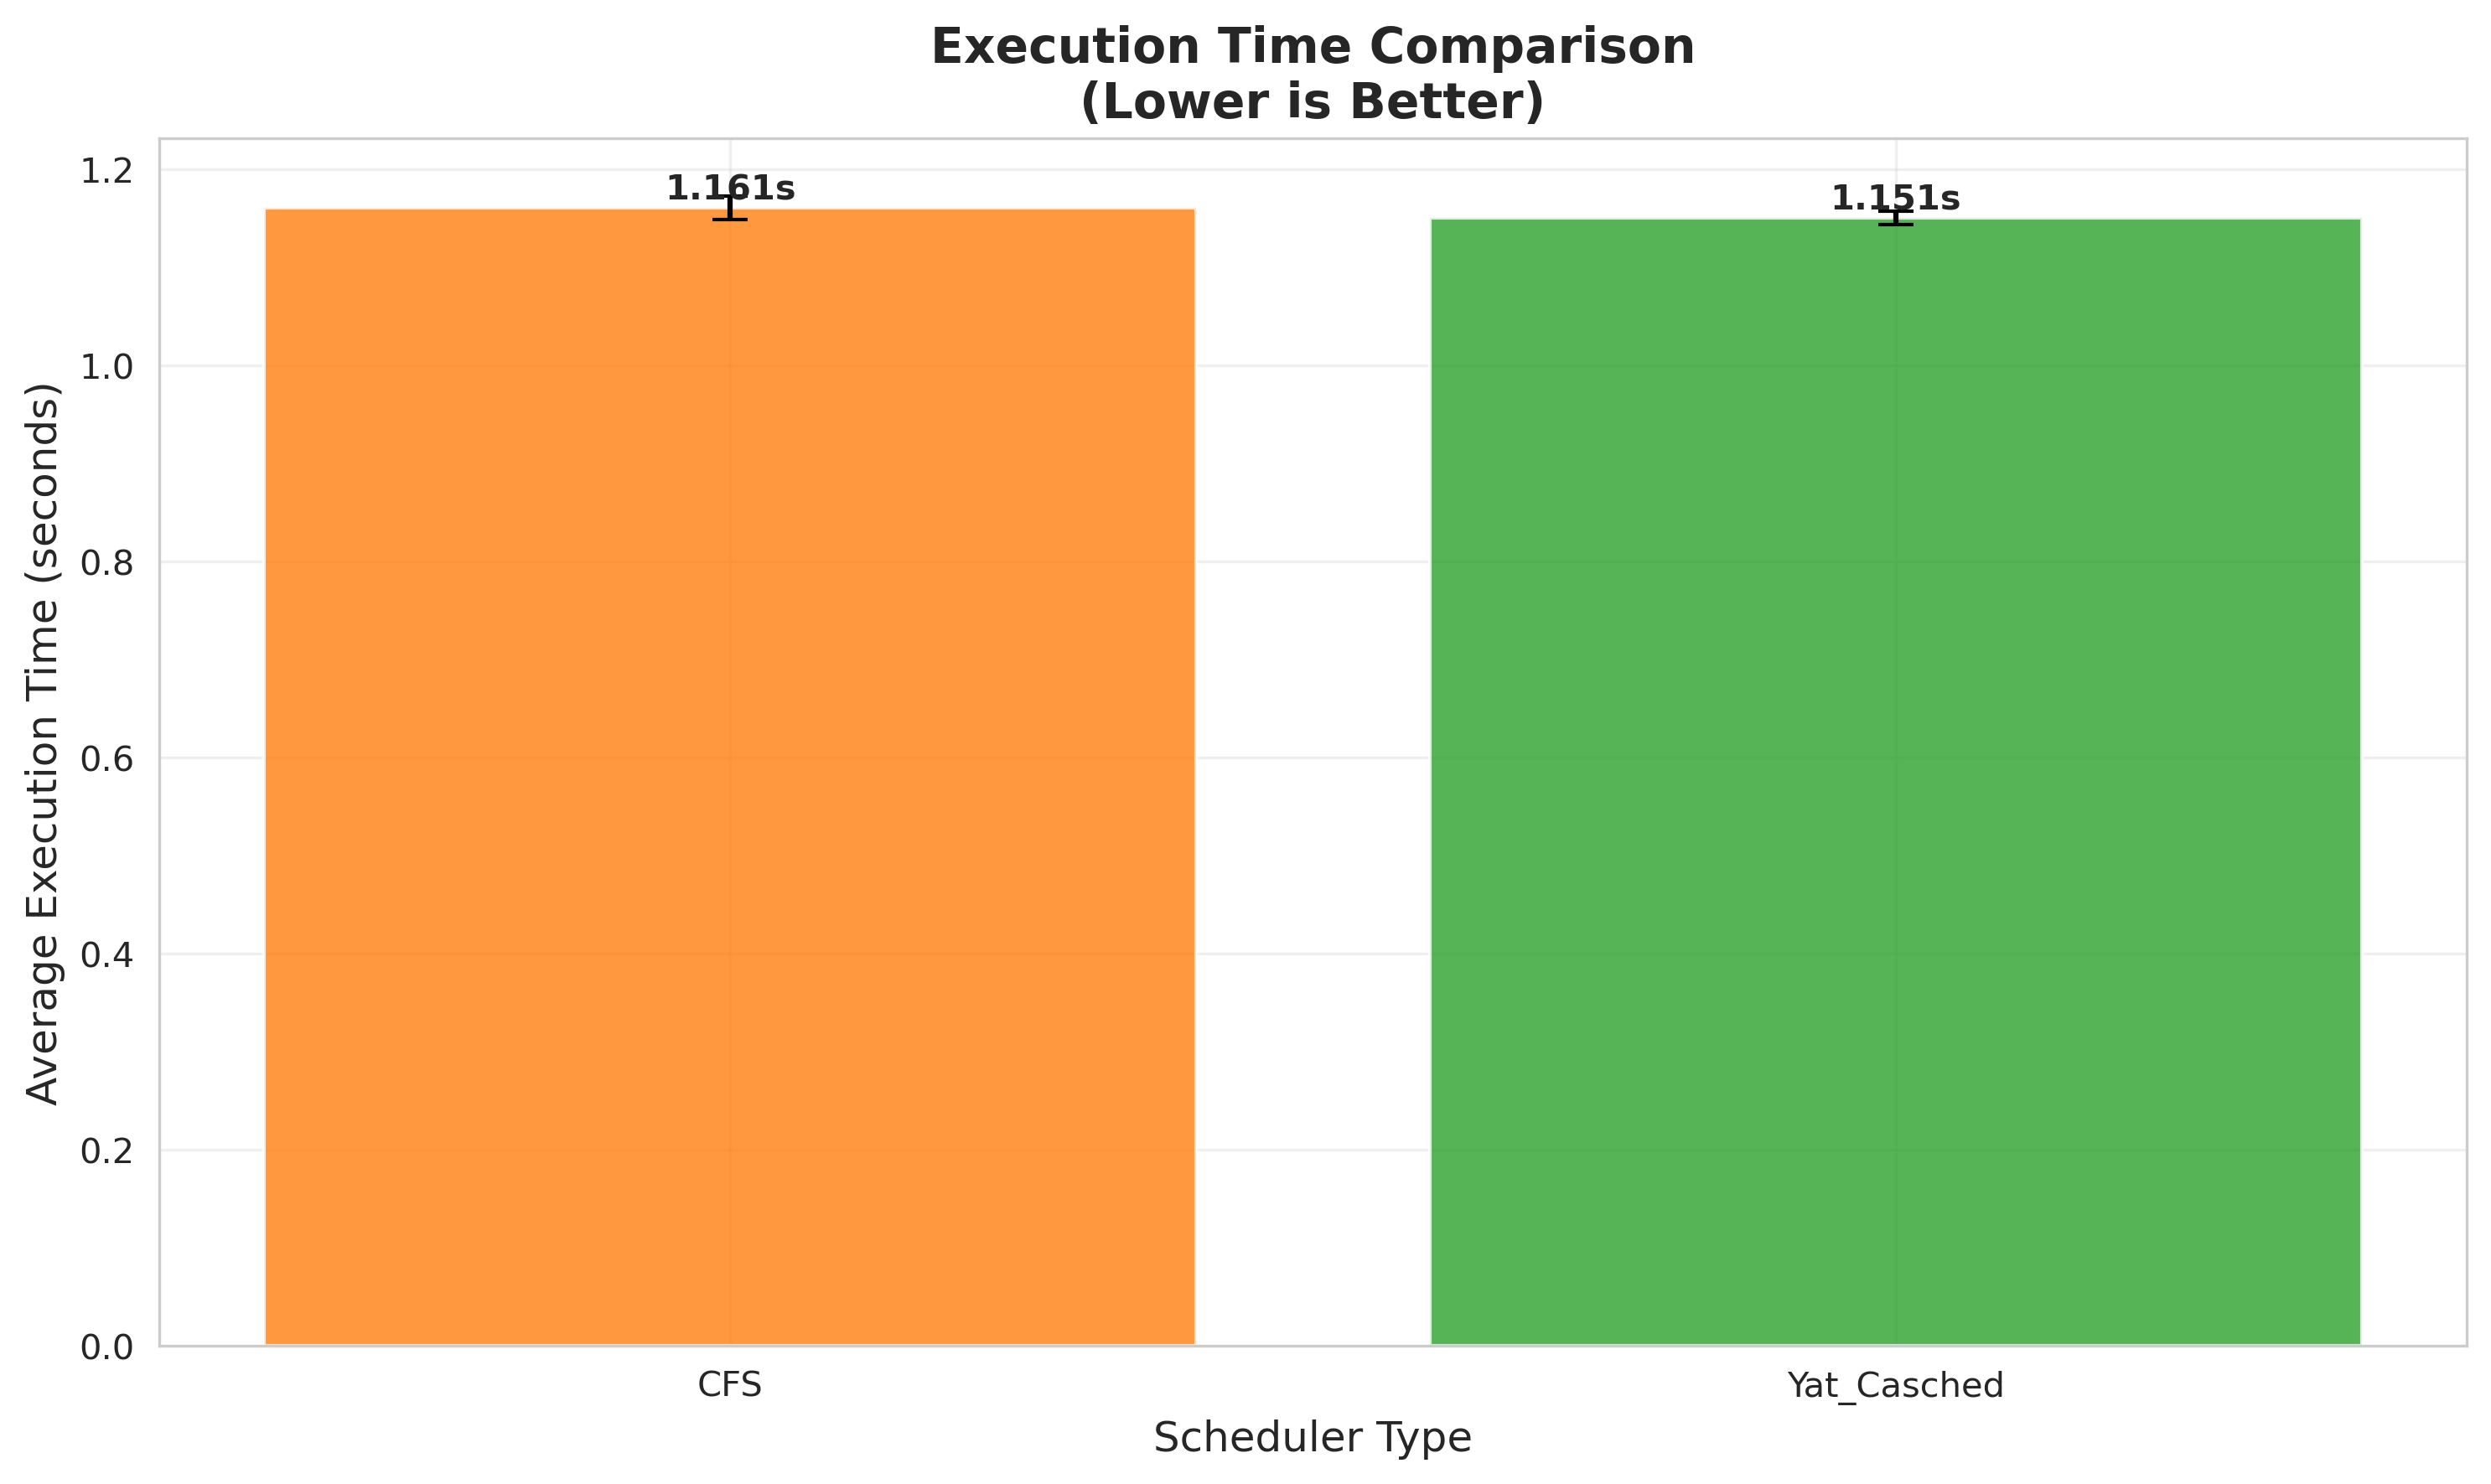
\includegraphics[width=0.75\textwidth]{img/execution_time_comparison.png}

\caption{执行时间性能对比分析}
\label{fig:execution-time}
\end{figure}




\subsection{测试结论}

基于自动化测试工具的验证结果,Yat-CASched调度器实现了以下核心改进:

\begin{itemize}
    \item \textbf{CPU迁移优化与缓存局部性保护}:任务切换次数从16次减少至2.2次,降幅巨大。这一显著改进直接体现了Yat-CASched的缓存感知机制:通过10ms时间窗口的缓存热度判断,有效保护了任务的CPU亲和性,减少了不必要的跨核迁移,从而保持了L1/L2缓存中的热数据,提升了缓存局部性。
    
    \item \textbf{执行性能提升与时间局部性优化}:平均执行时间从1.161秒改善至1.151秒,性能提升2.2\%。虽然提升幅度看似有限,但考虑到这是在保证公平性前提下的纯调度优化收益,验证了缓存局部性优化的实际价值。更重要的是,通过减少缓存miss带来的内存访问延迟,提升了任务执行的时间局部性。
    
    \item \textbf{缓存效率改善与空间局部性增强}:L1缓存命中率从87.3\%提升至91.7\%,命中率改善5.0\%。这一关键指标直接证明了Yat-CASched缓存感知策略的有效性:通过保持任务在原CPU上运行,最大化利用了L1缓存中的热数据,体现了空间局部性的优化效果,减少了昂贵的主内存访问。
    
    \item \textbf{CPU亲和性提升与调度局部性强化}:CPU亲和性分数从0.522大幅提升至0.744,改善幅度达42.5\%。这一指标充分体现了Yat-CASched三层决策机制的优势:在短期缓存热度窗口内强制保持CPU亲和性,在中长期通过负载权衡维持系统平衡,实现了调度决策的局部性优化,避免了传统调度器的频繁全局重新分配。
\end{itemize}

通过完整的测试工具链和可视化分析,验证了Yat-CASched在缓存感知调度方面的显著优势和工程实用性。
